%
% A header that lets you compile a chapter by itself, or inside a larger document.
% Adapted from http://stackoverflow.com/questions/3655454/conditional-import-in-latex
%
%
%Use \inbpdocument and \outbpdocument in your individual files, in place of \begin{document} and \end{document}. In your main file, put in a \def \ismaindoc {} before including or importing anything.
%
% David Duvenaud
% June 2011
% 
% ======================================
%
%


\ifx\ismaindoc\undefined
	\newcommand{\inbpdocument}{
		\def \ismaindoc {}
		% Use this header if we are compiling by ourselves.
		\documentclass[a4paper,11pt,authoryear,index]{common/PhDThesisPSnPDF}
		
%\usepackage{draftwatermark}
%\SetWatermarkLightness{0.95}

% ******************************************************************************
% ****************************** Custom Margin *********************************

% Add `custommargin' in the document class options to use this section
% Set {innerside margin / outerside margin / topmargin / bottom margin}  and
% other page dimensions

\ifsetMargin
\else
    \RequirePackage[left=37mm,right=30mm,top=35mm,bottom=30mm]{geometry}
    \setFancyHdr % To apply fancy header after geometry package is loaded
\fi


%\chead{Unfinished draft}
%\cfoot{\texttt{Unfinished draft - compiled on \today{} at \currenttime}}

% *****************************************************************************
% ******************* Fonts (like different typewriter fonts etc.)*************

% Add `customfont' in the document class option to use this section

\ifsetFont
\else
    % Set your custom font here and use `customfont' in options. Leave empty to
    % load computer modern font (default LaTeX font).  

    \RequirePackage{libertine} 
\fi

% *****************************************************************************
% *************************** Bibliography  and References ********************

%\usepackage{cleveref} %Referencing without need to explicitly state fig /table

% Add `custombib' in the document class option to use this section
\ifsetBib % True, Bibliography option is chosen in class options
\else % If custom bibliography style chosen then load bibstyle here

   \RequirePackage[square, sort, numbers, authoryear]{natbib} % CustomBib

% If you would like to use biblatex for your reference management, as opposed to the default `natbibpackage` pass the option `custombib` in the document class. Comment out the previous line to make sure you don't load the natbib package. Uncomment the following lines and specify the location of references.bib file

% \RequirePackage[backend=biber, style=numeric-comp, citestyle=numeric, sorting=nty, natbib=true]{biblatex}
% \bibliography{References/references} %Location of references.bib only for biblatex

\fi


% changes the default name `Bibliography` -> `References'
\renewcommand{\bibname}{References}


% *****************************************************************************
% *************** Changing the Visual Style of Chapter Headings ***************
% Uncomment the section below. Requires titlesec package.

%\RequirePackage{titlesec}
%\newcommand{\PreContentTitleFormat}{\titleformat{\chapter}[display]{\scshape\Large}
%{\Large\filleft{\chaptertitlename} \Huge\thechapter}
%{1ex}{}
%[\vspace{1ex}\titlerule]}
%\newcommand{\ContentTitleFormat}{\titleformat{\chapter}[display]{\scshape\huge}
%{\Large\filleft{\chaptertitlename} \Huge\thechapter}{1ex}
%{\titlerule\vspace{1ex}\filright}
%[\vspace{1ex}\titlerule]}
%\newcommand{\PostContentTitleFormat}{\PreContentTitleFormat}
%\PreContentTitleFormat


% *****************************************************************************
% **************************** Custom Packages ********************************
% *****************************************************************************


% ************************* Algorithms and Pseudocode **************************

%\usepackage{algpseudocode} 


% ********************Captions and Hyperreferencing / URL **********************

% Captions: This makes captions of figures use a boldfaced small font. 
%\RequirePackage[small,bf]{caption}

\RequirePackage[labelsep=space,tableposition=top]{caption} 
%\renewcommand{\figurename}{Figure} %to support older versions of captions.sty
\captionsetup{belowskip=12pt,aboveskip=4pt}

% ************************ Formatting / Footnote *******************************

%\usepackage[perpage]{footmisc} %Range of footnote options 


% ****************************** Line Numbers **********************************

%\RequirePackage{lineno}
%\linenumbers

% ************************** Graphics and figures *****************************

%\usepackage{rotating}
%\usepackage{wrapfig}
%\usepackage{float}
\usepackage{subfig} %note: subfig must be included after the `caption` package. 


% ********************************* Table **************************************

%\usepackage{longtable}
%\usepackage{multicol}
%\usepackage{multirow}
%\usepackage{tabularx}


% ***************************** Math and SI Units ******************************

\usepackage{amsfonts}
\usepackage{amsmath}
\usepackage{amssymb}
%\usepackage{siunitx} % use this package module for SI units


% ******************************************************************************
% ************************* User Defined Commands ******************************
% ******************************************************************************

% *********** To change the name of Table of Contents / LOF and LOT ************

%\renewcommand{\contentsname}{My Table of Contents}
%\renewcommand{\listfigurename}{List of figures}
%\renewcommand{\listtablename}{List of tables}


% ********************** TOC depth and numbering depth *************************

\setcounter{secnumdepth}{2}
\setcounter{tocdepth}{2}

% ******************************* Nomenclature *********************************

% To change the name of the Nomenclature section, uncomment the following line

%\renewcommand{\nomname}{Symbols}


% ********************************* Appendix ***********************************

% The default value of both \appendixtocname and \appendixpagename is `Appendices'. These names can all be changed via: 

%\renewcommand{\appendixtocname}{List of appendices}
%\renewcommand{\appendixname}{Appndx}

		% All my custom preamble stuff.  Shouldn't overlap with anything in official-preamble


% Paths to figure and table directories.
\newcommand{\symmetryfigsdir}{figures/symmetries}
\newcommand{\topologyfiguresdir}{figures/topology}
\newcommand{\infinitefiguresdir}{figures/infinite}
\newcommand{\grammarfiguresdir}{figures/grammar}
\newcommand{\introfigsdir}{figures/intro}
\newcommand{\gplvmfiguresdir}{figures/gplvm}
\newcommand{\warpedfiguresdir}{figures/warped-mixtures}
\newcommand{\deeplimitsfiguresdir}{figures/deep-limits}
\newcommand{\quadraturefigsdir}{figures/quadrature}
\newcommand{\additivefigsdir}{figures/additive}
\newcommand{\decompfigsdir}{figures/decomp}
\newcommand{\examplefigsdir}{figures/worked-example}


\usepackage{bm}  % for warped mixtures - is this necessary?
\usepackage{booktabs}
\usepackage{tabularx}
\usepackage{multirow}
\usepackage{datetime}
\renewcommand{\tabularxcolumn}[1]{>{\arraybackslash}m{#1}}
\usepackage{relsize}
\usepackage{graphicx}
\usepackage{amsmath,amssymb,textcomp}
\usepackage{nicefrac}
\usepackage{amsthm}
\usepackage{tikz}
\usetikzlibrary{arrows}
\usetikzlibrary{calc}
\usepackage{nth}
\usepackage{rotating}
\usepackage{array}
\usepackage{fp}
\usepackage[hyperpageref]{backref}
\def\foo{\hspace{\fill}\mbox{}\linebreak[0]\hspace*{\fill}}
\renewcommand*{\backref}[1]{}
\renewcommand*{\backrefalt}[4]{%
\ifcase #1 %
%
\or
\foo(page #2)%
\else
\foo(pages #2)%
\fi
}

\usepackage{cleveref}
\crefname{equation}{equation}{equations}


%% For submission, make all render blank.
%%%%%%%%%%%%%%%%%%%%%%%%%%%%%%%%%%%%%%%%%%%%%%%%%%%%%%%%%%
%%%% EDITING HELPER FUNCTIONS  %%%%%%%%%%%%%%%%%%%%%%%%%%%
%%%%%%%%%%%%%%%%%%%%%%%%%%%%%%%%%%%%%%%%%%%%%%%%%%%%%%%%%%

%% NA: needs attention (rough writing whose correctness needs to be verified)
%% TBD: instructions for how to fix a gap ("Describe the propagation by ...")
%% PROBLEM: bug or missing crucial bit 

%% use \fXXX versions of these macros to put additional explanation into a footnote.  
%% The idea is that we don't want to interrupt the flow of the paper or make it 
%% impossible to read because there are a bunch of comments.

%% NA's (and TBDs, those less crucially) should be written so 
%% that they flow with the text.

\definecolor{WowColor}{rgb}{.75,0,.75}
\definecolor{SubtleColor}{rgb}{0,0,.50}

% inline
\newcommand{\NA}[1]{\textcolor{SubtleColor}{ {\tiny \bf ($\star$)} #1}}
\newcommand{\LATER}[1]{\textcolor{SubtleColor}{ {\tiny \bf ($\dagger$)} #1}}
\newcommand{\TBD}[1]{\textcolor{SubtleColor}{ {\tiny \bf (!)} #1}}
\newcommand{\PROBLEM}[1]{\textcolor{WowColor}{ {\bf (!!)} {\bf #1}}}

% as margin notes

\newcounter{margincounter}
\newcommand{\displaycounter}{{\arabic{margincounter}}}
\newcommand{\incdisplaycounter}{{\stepcounter{margincounter}\arabic{margincounter}}}

\newcommand{\fTBD}[1]{\textcolor{SubtleColor}{$\,^{(\incdisplaycounter)}$}\marginpar{\tiny\textcolor{SubtleColor}{ {\tiny $(\displaycounter)$} #1}}}

\newcommand{\fPROBLEM}[1]{\textcolor{WowColor}{$\,^{((\incdisplaycounter))}$}\marginpar{\tiny\textcolor{WowColor}{ {\bf $\mathbf{((\displaycounter))}$} {\bf #1}}}}

\newcommand{\fLATER}[1]{\textcolor{SubtleColor}{$\,^{(\incdisplaycounter\dagger)}$}\marginpar{\tiny\textcolor{SubtleColor}{ {\tiny $(\displaycounter\dagger)$} #1}}}

%\renewcommand{\LATER}[1]{}
%\renewcommand{\fLATER}[1]{}
%\renewcommand{\TBD}[1]{}
%\renewcommand{\fTBD}[1]{}
%\renewcommand{\PROBLEM}[1]{}
%\renewcommand{\fPROBLEM}[1]{}
%\renewcommand{\NA}[1]{}


% HUMBLE WORDS: shown slightly smaller when in normal text
% Thanks to Christian Steinruecken!

% HUMBLE WORDS: shown slightly smaller when in normal text
%
\makeatletter%
%\def\@humbleformat#1{{\fontsize{}{1em}\selectfont #1}}
%\def\@humbleformat#1{\textsmaller{#1}}%
\newlength{\nonHumbleHeight}
\def\@humbleformat#1{{\settoheight{\nonHumbleHeight}{#1}\resizebox{!}{0.94\nonHumbleHeight}{#1}}}%
\def\@idxhumbleformat#1{{\relscale{0.95}{#1}}}%
%\def\@humbleformat#1{{#1}}%
\def\declareHumble#1#2{%
  \expandafter\def\csname #1\endcsname{\@humbleformat{#2}}%
  \expandafter\def\csname s#1\endcsname{{#2}}%
  \expandafter\def\csname idx#1\endcsname{{\@idxhumbleformat{#2}}}%
}%
\def\humble#1{\@humbleformat{#1}}%
\def\idxhumble#1{\@idxhumbleformat{#1}}%
\makeatother%

% Convenient indexing for humble abbreviations
\def\humbleindex#1#2{\index{#1@\idxhumble{#1}}}



% TODO: Clean up duplicates
\declareHumble{ANOVA}{ANOVA}
\declareHumble{ARD}{ARD}
\declareHumble{BIC}{BIC}
\declareHumble{BMC}{BMC}
\declareHumble{bq}{BQ}
\declareHumble{CRP}{CRP}
\declareHumble{dirpro}{DP}
\declareHumble{HDMR}{HDMR}
\declareHumble{GAM}{GAM}
\declareHumble{GEM}{GEM}
\declareHumble{GMM}{GMM}
\declareHumble{gplvm}{GP-LVM}
\declareHumble{gpml}{GPML}
\declareHumble{GPML}{GPML}
\declareHumble{gprn}{GPRN}
\declareHumble{gpt}{GP}
\declareHumble{gp}{GP}
\declareHumble{HKL}{HKL}
\declareHumble{HMC}{HMC}
\declareHumble{ibp}{IBP}
\declareHumble{iGMM}{iGMM}
\declareHumble{iwmm}{iWMM}
\declareHumble{kCP}{CP}
\declareHumble{kCW}{CW}
\declareHumble{kC}{C}
\declareHumble{KDE}{KDE}
\declareHumble{kLin}{Lin}
\declareHumble{KPCA}{KPCA}
\declareHumble{kPer}{Per}
\declareHumble{kRQ}{RQ}
\declareHumble{kSE}{SE}
\declareHumble{kWN}{WN}
\declareHumble{Lin}{Lin}
\declareHumble{LBFGS}{L-BFGS}
\declareHumble{mcmc}{MCMC}
\declareHumble{MKL}{MKL}
\declareHumble{MLP}{MLP}
\declareHumble{MSE}{MSE}
\declareHumble{Per}{Per}
\declareHumble{RMSE}{RMSE}
\declareHumble{RQ}{RQ}
\declareHumble{SBQ}{SBQ}
\declareHumble{seard}{SE-ARD}
\declareHumble{sefull}{SE-\textnormal{full}}
\declareHumble{SEGP}{SE-GP}
\declareHumble{SE}{SE}
\declareHumble{SNR}{SNR}
\declareHumble{SSANOVA}{SS-ANOVA}
\declareHumble{SVM}{SVM}

\newcommand{\kSig}{\boldsymbol\sigma}

\def\subexpr{{\cal S}}
\def\baseker{{\cal B}}
\def\numWinners{k}

\def\ie{i.e.\ }
\def\eg{e.g.\ }
\def\etc{etc.\ }
\let\oldemptyset\emptyset
\let\emptyset 0




% Unify notation between neural-net land and GP-land.
\newcommand{\hphi}{h}
\newcommand{\hPhi}{\vh}
\newcommand{\walpha}{w}
\newcommand{\wboldalpha}{\bw}
\newcommand{\wcapalpha}{\vW}
\newcommand{\lengthscale}{w}

\newcommand{\layerindex}{\ell}



\newcommand{\gpdrawbox}[1]{
\setlength\fboxsep{0pt}
\hspace{-0.15in} 
\fbox{
\includegraphics[width=0.464\columnwidth]{\deeplimitsfiguresdir/deep_draws/deep_gp_sample_layer_#1}
}}



\newcommand{\procedurename}{ABCD}
\newcommand{\genText}[1]{{\sf #1}}



\newcommand{\asdf}{$^{\textnormal{th}}$}

\newcommand{\binarysum}{\sum_{\bf{x} \in \{0,1\}^D}}
\newcommand{\expect}{\mathbb{E}}
\newcommand{\expectargs}[2]{\mathbb{E}_{#1} \left[ {#2} \right]}
\newcommand{\var}{\mathbb{V}}
\newcommand{\varianceargs}[2]{\mathbb{V}_{#1} \left[ {#2} \right]}
\newcommand{\cov}{\operatorname{cov}}
\newcommand{\Cov}{\operatorname{Cov}}
\newcommand{\covargs}[2]{\cov \left[ {#1}, {#2} \right]}
\newcommand{\variance}{\mathbb{V}}
\newcommand{\vecop}[1]{\operatorname{vec} \left( {#1} \right)}

\newcommand{\covarianceargs}[2]{\Cov_{#1} \left[ {#2} \right]}
\newcommand{\colvec}[2]{\left[ \begin{array}{c} {#1} \\ {#2} \end{array} \right]}
\newcommand{\tbtmat}[4]{\left[ \begin{array}{cc} {#1} & {#2} \\ {#3} & {#4} \end{array} \right]}

%\newcommand{\covskinny}[2]{\var\!\left(#1\middle\vert#2\right)} 

\newcommand{\acro}[1]{{\humble{#1}}}
%\newcommand{\vect}[1]{\boldsymbol{#1}}
\newcommand{\vect}[1]{{\bf{#1}}}
\newcommand{\mat}[1]{\mathbf{#1}}
\newcommand{\pderiv}[2]{\frac{\partial #1}{\partial #2}}
\newcommand{\npderiv}[2]{\nicefrac{\partial #1}{\partial #2}}

\newcommand{\pha}{^{\phantom{:}}}

\newcommand{\argmin}{\operatornamewithlimits{argmin}}
\newcommand{\argmax}{\operatornamewithlimits{argmax}}

% The following designed for probabilities with long arguments

\newcommand{\Prob}[2]{P\!\left(\,#1\;\middle\vert\;#2\,\right)}
\newcommand{\ProbF}[3]{P\!\left(\,#1\!=\!#2\;\middle\vert\;#3\,\right)}
\newcommand{\p}[2]{p\!\left(#1\middle\vert#2\right)}
\newcommand{\po}[1]{p\!\left(#1\right)}
\newcommand{\pF}[3]{p\!\left(\,#1\!=\!#2\;\middle\vert\;#3\,\right)} 
\newcommand{\mean}[2]{{m}\!\left(#1\middle\vert#2\right)}



\newcommand{\valpha}{\boldsymbol{\alpha}}
\newcommand{\va}{\vect{a}}
\newcommand{\vA}{\vect{A}}
\newcommand{\vB}{\mat{B}}
\newcommand{\vb}{\vect{b}}
\newcommand{\vC}{\mat{C}}
\newcommand{\vc}{\vect{c}}
\newcommand{\vecf}{\boldsymbol{f}}
\newcommand{\vell}{\vect{\ell}}
\newcommand{\vepsilon}{\boldsymbol{\epsilon}}
\newcommand{\veps}{\boldsymbol{\epsilon}}
\newcommand{\ve}{\boldsymbol{\epsilon}}
\newcommand{\vf}{\vecf}
\newcommand{\vg}{\vect{g}}
\newcommand{\vh}{\vect{h}}
\newcommand{\vI}{\mat{I}}
\newcommand{\vK}{\mat{K}}
\newcommand{\vk}{\vect{k}}
\newcommand{\vL}{\mat{L}}
\newcommand{\vl}{\vect{l}}
\newcommand{\vmu}{\boldsymbol{\mu}}
\newcommand{\vone}{\vect{1}}
\newcommand{\vphi}{\boldsymbol{\phi}}
\newcommand{\vpi}{\boldsymbol{\pi}}
\newcommand{\vq}{\vect{q}}
\newcommand{\vR}{\mat{R}}
\newcommand{\vr}{\vect{r}}
\newcommand{\vsigma}{\boldsymbol{\sigma}}
\newcommand{\vSigma}{\mat{\Sigma}}
\newcommand{\vS}{\mat{S}}
\newcommand{\vs}{\vect{s}}
\newcommand{\vtheta}{\boldsymbol{\theta}}
\newcommand{\vu}{\vect{u}}
\newcommand{\vV}{\mat{V}}
\newcommand{\vW}{\mat{W}}
\newcommand{\vw}{\vect{w}}
\newcommand{\vX}{\mat{X}}
\newcommand{\vx}{\vect{x}}
\newcommand{\vY}{\mat{Y}}
\newcommand{\vy}{\vect{y}}
\newcommand{\vzero}{\vect{0}}
\newcommand{\vZ}{\mat{Z}}
\newcommand{\vz}{\vect{z}}


\newcommand{\netweights}{\alpha}
\newcommand{\vnetweights}{\valpha}

\newcommand{\He}{\mathcal{H}}
\newcommand{\normx}[2]{\left\|#1\right\|_{#2}}
\newcommand{\Hnorm}[1]{\normx{#1}{\He}}
\newcommand{\mmd}{{\rm MMD}}


\newcommand{\mf}{\bar{\vf}}

%\newcommand{\mf}{\mu} %{\bar{\ell}}
\newcommand{\lf}{f} % Likelihood function
\newcommand{\st}{_\star}

% from simpler log-bq writeup
\newcommand{\lftwo}{{\log \ell}}
\newcommand{\mftwo}{{\bar \ell}}
\newcommand{\loggp}{{\log\acro{GP}}}%| \bX, \vy )}}
\newcommand{\loggpdist}{{\acro{GP}(\lftwo)}}%| \vX, \vy )}}


\newcommand{\inv}{^{{\mathsmaller{-1}}}}
\newcommand{\tohalf}{^{{\mathsmaller{\nicefrac{1}{2}}}}}

\newcommand{\Normal}{\mathcal{N}}
\newcommand{\N}[3]{\mathcal{N}\!\left(#1 \middle| #2,#3\right)}
\newcommand{\Nt}[2]{\mathcal{N}\!\left(#1,#2\right)}
\newcommand{\NT}[2]{\mathcal{N}\!\left(#1,#2\right)}
\newcommand{\GPdist}[3]{\mathcal{GP}\!\left(#1 \, \middle| \, #2, #3 \right)}
\newcommand{\bN}[3]{\mathcal{N}\big(#1 \middle| #2,#3\big)}
\newcommand{\boldN}[3]{\text{\textbf{\mathcal{N}}}\big(#1;#2,#3\big)}
\newcommand{\ones}[1]{\mat{1}_{#1}}
\newcommand{\eye}[1]{\mat{E}_{#1}}
\newcommand{\tra}{^{\mathsf{T}}}
%\newcommand{\tra}{^{\top}}
%\mathsf{T}
\newcommand{\trace}{\operatorname{tr}}
\newcommand{\shift}{\operatorname{shift}}
\renewcommand{\mod}{\operatorname{mod}}
\newcommand{\deq}{:=}
\newcommand{\oneofk}{\operatorname{one-of-k}}
%\newcommand{\degree}{^\circ}

\newcommand{\GPt}[2]{\mathcal{GP}\!\left(#1,#2\right)}
%\newcommand{\GPt}[2]{\gp\!\left(#1,#2\right)}

\DeclareMathOperator{\tr}{tr}
\DeclareMathOperator{\chol}{chol}
\DeclareMathOperator{\diag}{diag}

\newenvironment{narrow}[2]{%
  \begin{list}{}{%
  \setlength{\topsep}{0pt}%
  \setlength{\leftmargin}{#1}%
  \setlength{\rightmargin}{#2}%
  \setlength{\listparindent}{\parindent}%
  \setlength{\itemindent}{\parindent}%
  \setlength{\parsep}{\parskip}}%
\item[]}{\end{list}}



\newcommand{\dist}{\ \sim\ }
\def\given{\,|\,}

% Table stuff
\newcolumntype{C}[1]{>{\centering\let\newline\\\arraybackslash\hspace{0pt}}m{#1}}
\newcolumntype{L}[1]{>{\raggedright\let\newline\\\arraybackslash\hspace{0pt}}m{#1}}
\newcolumntype{R}[1]{>{\raggedleft\let\newline\\\arraybackslash\hspace{0pt}}m{#1}}


\def\ie{i.e.\ }
\def\eg{e.g.\ }
\def\iid{i.i.d.\ }
%\def\simiid{\sim_{\mbox{\tiny iid}}}
\def\simiid{\overset{\mbox{\tiny iid}}{\sim}}
\def\simind{\overset{\mbox{\tiny \textnormal{ind}}}{\sim}}
\def\eqdist{\stackrel{\mbox{\tiny d}}{=}}
%\newcommand{\distas}[1]{\mathbin{\overset{#1}{\kern \z@ \sim}}}
%TODO: fix this - it worked outside the thesis!
\newcommand{\distas}[1]{\mathbin{\overset{#1}{\sim}}}

\def\Reals{\mathbb{R}}

\def\Uniform{\mbox{\rm Uniform}}
\def\Bernoulli{\mbox{\rm Bernoulli}}
\def\GP{\mathcal{GP}}
\def\GPLVM{\mathcal{GP-LVM}}




% Kernel stuff

\def\iva{\vect{\inputVar}}
\def\ivaone{\inputVar}
\def\inputVar{x}
\def\InputVar{X}
\def\InputSpace{\mathcal{X}}
\def\outputVar{y}
\def\OutputSpace{\mathcal{Y}}
\def\function{f}
\def\kernel{k}
\def\KernelMatrix{K}
\def\SumKernel{\sum}
\def\ProductKernel{\prod}
\def\expression{e}
\def\feat{\vh}

\newcommand{\kerntimes}{ \! \times \!}
\newcommand{\kernplus}{ \, + \,}


% Proof stuff
\theoremstyle{plain}
\newtheorem{theorem}{Theorem}[section]
\newtheorem{lemma}[theorem]{Lemma}
\newtheorem{prop}[theorem]{Proposition}
\newtheorem{proposition}{Proposition}
\newtheorem*{cor}{Corollary}

% For infinite bq
\newcommand{\iv}{\theta}
\newcommand{\viv}{\vtheta}

% For intro chapter
\newcommand{\funcval}{\vf(\vX)}
\newcommand{\testpoint}{{\vx^\star}}

\newcommand{\underwrite}[2]{{\underbrace{#1}_{\textnormal{#2}}}}



% For kernel figures
\newcommand{\fhbig}{2cm}%
\newcommand{\fwbig}{3cm}%
\newcommand{\kernpic}[1]{\includegraphics[height=\fhbig,width=\fwbig]{\grammarfiguresdir/structure_examples/#1}}%
\newcommand{\kernpicr}[1]{\rotatebox{90}{\includegraphics[height=\fwbig,width=\fhbig]{\grammarfiguresdir/structure_examples/#1}}}%
\newcommand{\addkernpic}[1]{{\includegraphics[height=\fhbig,width=\fwbig]{\grammarfiguresdir/additive_multi_d/#1}}}%
\newcommand{\largeplus}{\tabbox{{\Large+}}}%
\newcommand{\largeeq}{\tabbox{{\Large=}}}%
\newcommand{\largetimes}{\tabbox{{\Large$\times$}}}%
\newcommand{\fixedx}{$x$ (with $x' = 1$)}%


		% ************************ Thesis Information & Meta-data **********************

%% The title of the thesis
%\title{Structured Gaussian Process Models} 
%\title{Automatic Model Construction \\ through \\ Structured Gaussian Processes}
%\title{Automatic Model-Building \\ through \\ Structured Gaussian Processes}
%\title{Automatic Modeling \\ with \\ Structured Gaussian Processes}    
\title{Automatic Model Construction \\ with Gaussian Processes}
%\title{Automatic Model Construction}
%\title{Automating Statistical Model Construction}


%\texorpdfstring is used for PDF metadata. Usage:
%\texorpdfstring{LaTeX_Version}{PDF Version (non-latex)} eg.,
%\texorpdfstring{$sigma$}{sigma}

%% The full name of the author
\author{David Kristjanson Duvenaud}

%% Department (eg. Department of Engineering, Maths, Physics)
%\dept{Department of Engineering}

%% University and Crest
\university{University of Cambridge}
\crest{
\includegraphics[width=0.25\textwidth]{University_Crest}}

%% You can redefine the submission text:
% Default as per the University guidelines: This dissertation is submitted for
% the degree of Doctor of Philosophy
%\renewcommand{\submissiontext}{change the default text here if needed}

%% Full title of the Degree 
\degree{Doctor of Philosophy}
 
%% College affiliation (optional)
\college{Pembroke College}

%% Submission date
\degreedate{June 2014} 

%% Meta information
\subject{LaTeX} \keywords{{LaTeX} {PhD Thesis} {Engineering} {University of Cambridge}}



		\begin{document}
	}	
	\newcommand{\outbpdocument}[1]{

		% Fake chapters so references aren't broken
\label{ch:intro}                
\label{ch:kernels}
\label{ch:grammar}
\label{ch:description}
\label{ch:additive}
\label{ch:deeplimits}
\label{ch:discussion}
		%\bibliographystyle{common/CUEDthesis}
		\bibliographystyle{plainnat}
		\bibliography{references.bib}
		\end{document}
	}	
\else
	%If we're inside another document, no need to re-start the document.
	\ifx\inbpdocument\undefined
		\newcommand{\inbpdocument}{}
		\newcommand{\outbpdocument}[1]{}
	\fi
\fi

\inbpdocument


\chapter{Characterizing Deep Gaussian Process Models}
\label{ch:deep-limits}

\begin{quotation}
``On a given day, would I rather be wrestling with a sampler, or proving theorems?''

\hspace*{\fill} \emph{Peter Orbanz}, personal communication
\end{quotation}




Choosing appropriate architectures and regularization strategies of deep networks is crucial to good predictive performance.  To shed light on this problem, we analyze the analogous problem of constructing useful priors on compositions of functions.  Specifically, we study the deep Gaussian process, a type of infinitely-wide, deep neural network.  We show that in standard architectures, the representational capacity of the network tends to capture fewer degrees of freedom as the number of layers increases, retaining only a single degree of freedom in the limit.  We propose an alternate network architecture which does not suffer from this pathology.  We also examine deep covariance functions, obtained by composing infinitely many feature transforms.  Lastly, we characterize the class of models obtained by performing dropout on Gaussian processes.

%This chapter was joint work with Oren Rippel, Ryan P. Adams and Zoubin Ghahramani.





\section{Introduction}

Much recent work on deep networks has focused on weight initialization \citep{martens2010deep}, regularization \citep{lee2007sparse} and network architecture \citep{gens2013learning}.
However, the interactions between these different design decisions can be complex and difficult to characterize.
We propose to approach the design of deep architectures by examining the problem of assigning priors to nested compositions of functions.
% Although inference in fully Bayesian models is generally challenging, well-defined priors allow us to encode our beliefs into models in a data-independent way. 
Well-defined priors allow us to explicitly examine the assumptions being made about functions we may wish to learn.
If we can identify classes of priors that give our models desirable properties, these in turn may suggest regularization, initialization, and architecture choices that also provide such properties.

Fundamentally, a multilayer neural network implements a composition of vector-valued functions, one per layer.
Hence, understanding properties of such function compositions helps us gain insight into deep networks.
In this paper, we examine a simple and flexible class of priors on compositions of functions, namely deep Gaussian processes \citep{damianou2012deep}.
Deep \gp{}s are simply priors on compositions of vector-valued functions, where each output of each layer is drawn independently from a GP prior:
%
\begin{align}
\vf^{(1:L)}(\vx) & = \vf^{(L)}(\vf^{(L-1)}(\dots \vf^{(2)}(\vf^{(1)}(\vx)) \dots)) \\
\vf_d^{(\layerindex)} & \simind \gp{} \left( 0, k^\layerindex_d(\vx, \vx') \right)
\label{eq:deep-gp}
\end{align}
%
%Although inference in these models is non-trivial,
These models correspond to a certain type of infinitely-wide multi-layer perceptron (\MLP{}), and as such make canonical candidates for generative models of functions that closely relate to neural networks.

By characterizing these models, this paper shows that representations based on repeated composition of independently-initialized functions exhibit a pathology where the representation becomes invariant to all but one direction of variation. This corresponds to an eventual debilitating decrease in the information capacity of networks as a function of their number of layers. However, we will demonstrate that a simple change in architecture --- namely, connecting the input to each layer --- fixes this problem. 

We also present two related analyses:  first, we examine the properties of a arbitrarily deep fixed feature transforms (``deep kernels'').  Second, we characterise the prior obtained by performing dropout on \gp{}s, showing equivalences to existing models.

%Section \ref{sec:relating} will derive the precise relationship between deep \gp{}s and MLPs.  Section \ref{sec:1d} will examine the asymptotic behavior of arbitrarily deep one-dimensional \gp{}s.  Section \ref{sec:theorem} gives a theorem characterizing the Jacobian of a deep multidimensinal \gp{}.  Section 
%Deep networks have become an important tool for machine learning [cite].  However, training these models are difficult, Many arguments have been made for the need for deep architectures [cite Bengio].  However, it is hard to know what effect the deepness of an architecture has.  Also, the weights don't necessarily move that much from their initialization.

%Good initialization schemes can help, but we are interested in creating distributions on deep functions so that most of the mass is on functions without any pathologies.  Also, we might be able to show that the pathologies we show that most functions exhibit means that it will be hard to learn them by gradient descent.







\section{Relating deep neural nets and deep Gaussian processes}
\label{sec:relating}
%There are two ways to view deep Gaussian processes as neural networks.  First, we can
%We introduce a generative non-parametric model to address this problem.  Our approach is based on the GP-LVM ~\cite{lawrence2004gaussian,salzmann2008local,lawrence2009non}, a flexible nonparametric density model.  

%\cite{NIPS2005_424} showed that kernel machines such as \gp{}s have limited generalization ability when they are forced to use a 'local' kernel.

%\subsection{A neural net with one hidden layer}
%\vspace{-0.05in}
\subsection{Single-layer models}

\begin{figure}
\def\layersep{1.33cm}
\def\nodesep{.75cm}
\def\nodesize{.35cm}

%\newcommand{\numdims}[0]{3}
%\newcommand{\numhidden}[0]{4}
%\newcommand{\upnodedist}[0]{0.6cm}
%\newcommand{\bardist}[0]{\hspace{-0.2cm}}

\begin{tabular}{c|c|c}
\hspace{-0.5cm}
\begin{tikzpicture}[shorten >=1pt,->,draw=black!50, node distance=\layersep]
    \tikzstyle{every pin edge}=[<-,shorten <=1pt]
    \tikzstyle{neuron}=[circle,fill=black!25,minimum size=17pt,inner sep=0pt]
    \tikzstyle{input neuron}=[neuron, fill=green!50];
    \tikzstyle{output neuron}=[neuron, fill=red!50];
    \tikzstyle{hidden neuron}=[neuron, fill=blue!50];
    \tikzstyle{annot} = [text width=4em, text centered]

    % Draw the input layer nodes
    \foreach \name / \y in {1,...,\numdims}
    % This is the same as writing \foreach \name / \y in {1/1,2/2,3/3,4/4}
        \node[input neuron, minimum size=\nodesize
        %, pin=left:Input \#\y
        ] (I-\name) at (0,-\nodesep*\y) {}; %{$x_\y$};

    % Draw the hidden layer nodes
    \foreach \name / \y in {1,...,\numhidden}
        \path[yshift=0.5cm]
            node[hidden neuron, minimum size=\nodesize] (H-\name) at (\layersep,-\nodesep*\y) {}; %{$\phi_\y$};

    % Draw the output layer node
    \foreach \name / \y in {1,...,\numdims}
    	\node[output neuron, minimum size=\nodesize
    	%,pin={[pin edge={->}]right:Output }
    	] (O-\name) at (2*\layersep,-\nodesep*\y) {};%{$f^{1}_\y$};

    % Connect every node in the input layer with every node in the
    % hidden layer.
    \foreach \source in {1,...,\numdims}
        \foreach \dest in {1,...,\numhidden}
            \path (I-\source) edge (H-\dest);

    % Connect every node in the hidden layer with the output layer
    \foreach \source in {1,...,\numhidden}
        \foreach \dest in {1,...,\numdims}
    	    \path (H-\source) edge (O-\dest);

    % Annotate the layers
    \node[annot,above of=I-1, node distance=\upnodedist] {Inputs};
    \node[annot,above of=H-1, node distance=\upnodedist] {Hidden};
    \node[annot,above of=O-1, node distance=\upnodedist] {Outputs};
\end{tikzpicture}
\bardist
&
\bardist
\begin{tikzpicture}[shorten >=1pt,->,draw=black!50, node distance=\layersep]
    \tikzstyle{every pin edge}=[<-,shorten <=1pt]
    \tikzstyle{neuron}=[circle,fill=black!25,minimum size=17pt,inner sep=0pt]
    \tikzstyle{input neuron}=[neuron, fill=green!50];
    \tikzstyle{output neuron}=[neuron, fill=red!50];
    \tikzstyle{hidden neuron}=[neuron, fill=blue!50];
    \tikzstyle{annot} = [text width=4em, text centered]

    % Draw the input layer nodes
    \foreach \name / \y in {1,...,\numdims}
    % This is the same as writing \foreach \name / \y in {1/1,2/2,3/3,4/4}
        \node[input neuron, minimum size=\nodesize
        %, pin=left:Input \#\y
        ] (I-\name) at (0,-\nodesep*\y) {};

    % Draw the hidden layer nodes
    \foreach \name / \y in {1,...,\numhidden}
        \path[yshift=0.5cm]
            node[hidden neuron, minimum size=\nodesize] (H-\name) at (\layersep,-\nodesep*\y) {};

    % Draw the hidden layer nodes
    \foreach \name / \y in {1,...,\numhidden}
        \path[yshift=0.5cm]
            node[hidden neuron, minimum size=\nodesize] (H2-\name) at (2*\layersep,-\nodesep*\y) {};


    % Draw the output layer node
    \foreach \name / \y in {1,...,\numdims}
    	\node[output neuron, minimum size=\nodesize
    	%,pin={[pin edge={->}]right:Output }
    	] (O-\name) at (3*\layersep,-\nodesep*\y) {};

    % Connect every node in the input layer with every node in the
    % hidden layer.
    \foreach \source in {1,...,\numdims}
        \foreach \dest in {1,...,\numhidden}
            \path (I-\source) edge (H-\dest);
            
    \foreach \source in {1,...,\numhidden}
        \foreach \dest in {1,...,\numhidden}
            \path (H-\source) edge (H2-\dest);            

    % Connect every node in the hidden layer with the output layer
    \foreach \source in {1,...,\numhidden}
        \foreach \dest in {1,...,\numdims}
    	    \path (H2-\source) edge (O-\dest);

    % Annotate the layers
    \node[annot,above of=I-1, node distance=\upnodedist] {Inputs};
    \node[annot,above of=H-1, node distance=\upnodedist] {Hidden};
    \node[annot,above of=H2-1, node distance=\upnodedist] {Hidden};
    \node[annot,above of=O-1, node distance=\upnodedist] {Outputs};
\end{tikzpicture}
\bardist
&
\bardist
\begin{tikzpicture}[shorten >=1pt,->,draw=black!50, node distance=\layersep]
    \tikzstyle{every pin edge}=[<-,shorten <=1pt]
    \tikzstyle{neuron}=[circle,fill=black!25,minimum size=17pt,inner sep=0pt]
    \tikzstyle{input neuron}=[neuron, fill=green!50];
    \tikzstyle{output neuron}=[neuron, fill=red!50];
    \tikzstyle{hidden neuron}=[neuron, fill=blue!50];
    \tikzstyle{annot} = [text width=4em, text centered]

    % Draw the input layer nodes
    \foreach \name / \y in {1,...,\numdims}
    % This is the same as writing \foreach \name / \y in {1/1,2/2,3/3,4/4}
        \node[input neuron, minimum size=\nodesize
        %, pin=left:Input \#\y
        ] (I-\name) at (0,-\nodesep*\y) {};

    % Draw the hidden layer nodes
    \foreach \name / \y in {1,...,\numhidden}
        \path[yshift=0.5cm]
            node[hidden neuron, minimum size=\nodesize] (H-\name) at (\layersep,-\nodesep*\y) {};

    % Draw the hidden layer nodes
    \foreach \name / \y in {1,...,\numhidden}
        \path[yshift=0.5cm]
            node[hidden neuron, minimum size=\nodesize] (H2-\name) at (3*\layersep,-\nodesep*\y) {};

    % Draw the output layer node
    \foreach \name / \y in {1,...,\numdims}
    	\node[output neuron, minimum size=\nodesize
    	%,pin={[pin edge={->}]right:Output }
    	] (O1-\name) at (2*\layersep,-\nodesep*\y) {};

    % Draw the output layer node
    \foreach \name / \y in {1,...,\numdims}
    	\node[output neuron, minimum size=\nodesize
    	%,pin={[pin edge={->}]right:Output }
    	] (O2-\name) at (4*\layersep,-\nodesep*\y) {};

    % Connect every node in the input layer with every node in the
    % hidden layer.
    \foreach \source in {1,...,\numdims}
        \foreach \dest in {1,...,\numhidden}
            \path (I-\source) edge (H-\dest);
            
    \foreach \source in {1,...,\numhidden}
        \foreach \dest in {1,...,\numdims}
            \path (H-\source) edge (O1-\dest);         
            
    \foreach \source in {1,...,\numdims}
        \foreach \dest in {1,...,\numhidden}
            \path (O1-\source) edge (H2-\dest);                

    % Connect every node in the hidden layer with the output layer
    \foreach \source in {1,...,\numhidden}
        \foreach \dest in {1,...,\numdims}
    	    \path (H2-\source) edge (O2-\dest);

    % Annotate the layers
    \node[annot,above of=I-1, node distance=\upnodedist] {Inputs};
    \node[annot,above of=H-1, node distance=\upnodedist] {Hidden};
    \node[annot,above of=O1-1, node distance=\upnodedist] {$\vf^{(1)}(\vx)$};
    \node[annot,above of=H2-1, node distance=\upnodedist] {Hidden};
    \node[annot,above of=O2-1, node distance=\upnodedist] {$\vf^{(1:2)}(\vx)$};

\end{tikzpicture} \\
\hspace{-0.5cm} a) One-hidden-layer MLP & 
b) Two-hidden layer MLP & 
\hspace{-0.3cm} c) Two-layer \gp{}: $\vy = \vf^{(2)} \left( \vf^{(1)}(\vx) \right)$
\end{tabular}
\caption[Comparison of neural network architectures]
{GPs can be understood as one-hidden-layer MLP with infinitely many hidden units (a).
There are two possible interpretations of deep GPs:
We can consider the deep \gpt{} to be a neural network with a finite number of hidden units, each with a different non-parametric activation function (b).
Alternatively, we can consider every second layer to be a random linear combination of an infinite number of fixed parametric hidden units (c).
}
\label{fig:architectures}
\end{figure}

In the typical definition of an \MLP{}, the hidden units of the first layer are defined as:
%
\begin{align}
\vh^{(1)}(\vx) = \sigma \left( \vb^{(1)} + \vW^{(1)}\vx \right)
\end{align}
%
where $\vh$ are the hidden unit activations, $\vb$ is a bias vector, $\vW$ is a weight matrix and $\sigma$ is a one-dimensional nonlinear function applied element-wise. The output vector $f(\vx)$ is simply a weighted sum of these hidden unit activations:
%
\begin{align}
f(\vx) = \vV^{(1)} \sigma \left( \vb^{(1)} + \vW^{(1)} \vx \right)  = \vV^{(1)} \vh^{(1)}(\vx)
\label{eq:one-layer-nn}
\end{align}
%
where $\vV^{(1)}$ is another weight matrix.

There exists a correspondence between one-layer \MLP{}s and \gp{}s \citep{neal1995bayesian}.  \gp{}s can be viewed as a prior on neural networks with infinitely many hidden units, and unknown weights.  More precisely, for any model of the form
%
\begin{align}
f(\vx) = \frac{1}{K}{\mathbf \alpha}\tra \hPhi(\vx) = \frac{1}{K} \sum_{i=1}^K \alpha_i \hphi_i(\vx),
\label{eq:one-layer-gp}
\end{align}
%
with fixed features $\left[ \hphi_1(\vx), \dots, \hphi_K(\vx) \right]\tra = \hPhi(\vx)$ and i.i.d. $\alpha$'s with zero mean and finite variance $\sigma^2$, the central limit theorem implies that as the number of features $K$ grows, any two function values $f(\vx), f(\vx')$ have a joint distribution approaching $\Nt{0}{\frac{\sigma^2}{K}\sum_{i=1}^K \hphi_i(\vx)\hphi_i(\vx')}$.
A joint Gaussian distribution between any set of function values is the definition of a Gaussian process.
%\TBD{DD: any two or any set?}

The result is surprisingly general:
it puts no constraints on the features (other than having uniformly bounded activation), nor does it require that the feature weights $\alpha$ be Gaussian distributed.  

We can also work backwards to derive a one-layer \MLP{} from any \gp{}.
Mercer's theorem implies that any positive-definite kernel function corresponds to an inner product of features: $k(\vx, \vx') = \hPhi(\vx) \tra \hPhi(\vx')$.
%
Thus in the one-hidden-layer case, the correspondence between \MLP{}s and \gp{}s is simple:
the features $\hPhi(\vx)$ of the kernel correspond to the hidden units of the \MLP{}.


\subsection{Multiple hidden layers}

%\paragraph{Fixed nonlinearities}
In an \MLP{}, the $\layerindex$th layer units are given by the recurrence
%
\begin{align}
\vh^{(\layerindex)}(\vx) = \sigma \left( \vb^{(\layerindex)} + \vW^{(\layerindex)} \vh^{(\layerindex-1)}(\vx) \right) \;.
\label{eq:nextlayer}
\end{align}
This architecture is shown in figure \ref{fig:architectures}b. 
%In this model, each hidden layer's output feeds directly into the next layer's input, weighted by the corresponding element of $\vW^{(\layerindex)}$.  
%
For example, if we extend the model given by \eqref{eq:one-layer-nn} to have two layers of feature mappings,  the resulting model is
%
\begin{align}
f(\vx) = \frac{1}{K}{\mathbf \alpha}\tra \hPhi^{(2)}\left( \hPhi^{(1)}(\vx) \right) \;.
% = \frac{1}{K} \sum_{i=1}^K \alpha_i \hphi_i(\vx),
\label{eq:mutli-layer-nn}
\end{align}

If the features $\vh(\vx)$ are considered fixed with only the last layer weights ${\mathbf \alpha}$ unknown, this model corresponds to a \gp{} with a ``deep kernel'': 
\begin{align}
k(\vx, \vx') = \left( \hPhi^{(2)} ( \hPhi^{(1)}(\vx) ) \right) \tra \hPhi^{(2)} (\hPhi^{(1)}(\vx') )
\end{align}
These models, examined in section \ref{sec:deep_kernels}, imply a fixed representation as opposed to a prior over representations, which is what we wish to analyze in this paper.


%In a neural net with multiple hidden layers, the correspondence is a little more complicated.
 

To construct a neural network with fixed nonlinearities corresponding to a deep \gp{}, 
%with $D_\layerindex$ units for each layer corresponding to the outputs compositions of functions drawn from a \gp{} prior, 
one must introduce a second layer in between each infinitely-wide set of fixed basis functions, as in figure \ref{fig:architectures}c.
The $D_\layerindex$ outputs $\vf^{(\layerindex)}(\vx)$ in between each layer are weighted sums (with unknown weights) of the fixed hidden units of the layer below, and the next layer's hidden units depend only on these $D_\layerindex$ outputs.
%Thus, the network architecture with fixed nonlinearities corresponding to deep \gp{}s has an extra set of layers that a \MLP{} doesn't have.
%

This alternating-layer architecture has an interpretation as a series of linear information bottlenecks.
We can simply substitute \eqref{eq:one-layer-nn} into \eqref{eq:nextlayer} to get
%
\begin{align}
\hPhi^{(\layerindex)}(\vx) = \sigma \left( \vb^{(\layerindex)} + \vW^{(\layerindex)} \vV^{(\layerindex-1)} \hPhi^{(\layerindex-1)}(\vx) \right) \;.
\end{align}
%
Thus, ignoring the intermediate outputs $\vf^{(\layerindex)}(\vx)$, a deep \gp{} is an infinitely-wide, deep \MLP{} with each pair of layers connected by random, rank-$D_\layerindex$ matrices $\vW^{(\layerindex)} \vV^{(\layerindex-1)}$. %connecting the layers.



%There are two ways to relate deep \gp{}s to \MLP{}s.
A more direct way to construct a network architecture corresponding to a deep \gp{} is to integrate out all $\vV^{(\layerindex)}$, and view deep \gp{}s as a neural network with a finite number of nonparametric, \gp{}-distributed basis functions at each layer, in which $\vf^{(1:\layerindex)}(\vx)$ represent the output of the hidden nodes at the $\layerindex^{th}$ layer.
This second view lets us compare deep \gp{} models to standard neural net architectures more directly.
%, examining the activations and shapes of the finite number of basis functions at each layer.


%Figure \ref{fig:architectures} compares these two architectures.  If we stick to the correspondence between neural nets and \gp{}s as defined in \eqref{eq:one-layer-nn}, we notice that the deep \gp{} architecture forces the linear connections between hidden layers go be squeezed through a finite set of nodes, corresponding to the output of the independent \gp{}s at each layer.  




%\subsection{Relating initialization strategies, regularization, and priors}

%Traditional training of deep networks requires both an an initialization strategy, and a regularization method.  In a Bayesian model, the prior implicitly defines both of these things.

%For example, one feature of \gp{} models with a clear analogue to initialization strategies in deep networks is automatic relevance determination. 
%\paragraph{The effects of automatic relevance determination}  One feature of Gaussian process models that doesn't have a clear anologue in the neural-net literature is automatic relevance determination (ARD).  Recall that 
%In the ARD procedure, the lengthscales of each dimension are scaled to maximize the marginal likelihood of the GP.  In standard one-layer GP regression, it has the effect of smoothing out the posterior over functions in directions in which the data does not change.

%\paragraph{Sparse Initialization}
%\cite{martens2010deep} used “sparse initialization”, in which each hidden unit had 15 non-zero incoming connections.  %They say ``this allows the units to be both highly differentiated as well as unsaturated, avoiding the problem in dense initializations where the connection weights must all be scaled very small in order to prevent saturation, leading to poor differentiation between units''.
%
%While it is not clear if deep GPs have analogous problems with saturation of connection weights, we note that 
%An anologous initialization strategy would be to put a heavy-tailed prior on the lengthscales in the squared-exp kernel.


%\subsection{What kinds of functions do deep GPs prefer?}
%Isotropic kernels such as the squared-exp encode the assumption that the function varies independently in all directions.  
%This implies that using an isotropic kernel to model a function that does \emph{not} vary in all direction independently is 'wasting marginal likelihood' by not making strong enough assumptions.  
%
%Thus, deep GPs prefer to have hidden layers on whose outputs the higher-layer functions vary independently.  In this way, we can say that the deep GP model prefers independent features.

%Combining these two properties of isotropic kernels, we can say that a deep GP will attempt to transform its input into a representation with as few degrees of freedom as possible, and for which the output function varies independently across each dimension.




\section{Characterizing deep Gaussian processes}
\label{sec:characterizing-deep-gps}

In this section, we develop several theoretical results that explore the behavior of deep \gp{}s as a function of their depth.  This will allow us in section \ref{sec:formalizing-pathology} to formally identify a pathology that emerges in very deep networks.

Specifically, we will show that the size of the derivative of a one-dimensional deep \gp{} becomes log-normal distributed as the network becomes deeper.  We'll also show that the Jacobian of a multivariate deep \gp{} is a product of independent Gaussian matrices with independent entries.


\subsection{One-dimensional asymptotics}
\label{sec:1d}

%One way to understand the properties of functions drawn from deep \gp{}s and deep networks is by looking at the distribution of the derivative of these functions. We first focus on the one-dimensional case.

In this section, we derive the limiting distribution of the derivative of an arbitrarily deep, one-dimensional \gp{} with a squared-exp kernel:  %in order to shed light on the ways in which a deep \gp{}s are non-Gaussian, and the ways in which lower layers affect the computation performed by higher layers.
%
\newcommand{\onedsamplepic}[1]{
\hspace{-0.25in}
\includegraphics[trim=2mm 2mm 2mm 6.4mm, clip, width=0.255\columnwidth]{\deeplimitsfiguresdir/1d_samples/latent_seed_0_1d_large/layer-#1}} 
%
\newcommand{\onedsamplepiccon}[1]{
\hspace{-0.25in}
\includegraphics[trim=2mm 2mm 2mm 6.4mm, clip, width=0.255\columnwidth]{\deeplimitsfiguresdir/1d_samples/latent_seed_0_1d_large_connected/layer-#1}} 
%
\begin{figure}
\centering
\begin{tabular}{cccc}
\hspace{-0.1in} 1 layer & \hspace{-0.2in} 2 Layers & 5 Layers & \hspace{-0.25in} 10 Layers \\
\hspace{0.03in}
\onedsamplepic{1} &
\onedsamplepic{2} &
\onedsamplepic{5} &
\onedsamplepic{10}
%& 6 layers \\ & largest , for unconnected layers & largest, for connected layers
\end{tabular}
\caption[One-dimensional draws from a deep gp prior]
{One-dimensional draws from a deep gp prior.
After a few layers, the functions begin to be either nearly flat, or highly varying, everywhere.
This is a consequence of the distribution on derivatives becoming heavy-tailed.}
\label{fig:deep_draw_1d}
\end{figure}
%
\begin{align}
k_{\textnormal{SE}}(x, x') = \sigma^2 \exp \left( \frac{-(x - x')^2}{2\lengthscale^2} \right) \;.
\label{eq:se_kernel}
\end{align}
%
The hyperparameter $\sigma^2$ controls the variance of functions drawn from the prior, and the hyperparameter $\lengthscale$ controls the smoothness.  
The derivative of a \gp{} with a squared-exp kernel is pointwise distributed as $\Nt{0}{\nicefrac{\sigma^2}{\lengthscale^2}}$.  
Intuitively, a \gp{} is likely to have large derivatives if it has high variance and small lengthscales.
 
 By the chain rule, the derivative of a one-dimensional deep \gp{} is simply a product of its (independent) derivatives.  
 The distribution of the absolute value of this derivative is a product of half-normals, each with mean $\sqrt{\nicefrac{2 \sigma^2}{\pi \lengthscale^2}}$.
%
%\begin{align}
%\frac{\partial f(x)}{\partial x} & \distas{iid} \Nt{0}{\frac{\sigma^2_f}{\lengthscale^2}} \\
%\implies 
%\left| \frac{\partial f(x)}{\partial x} \right| & \distas{iid} \textnormal{half}\Nt{\sqrt{\frac{2 \sigma^2_f}{\pi\lengthscale^2}}}{\frac{\sigma^2_f}{\lengthscale^2} \left( 1 - \frac{2}{\pi} \right)}
%\end{align}

If we choose kernel parameters so that ${\nicefrac{\sigma^2}{\lengthscale^2} = \nicefrac{\pi}{2}}$, then the expected magnitude of the derivative remains constant regardless of the depth.

%then ${\expectargs{}{\left| \nicefrac{\partial f(x)}{\partial x} \right|} = 1}$, and so ${\expectargs{}{\left| \nicefrac{\partial f^{(1:L)}(x)}{\partial x} \right|} = 1}$ for any $L$.
%  If $\nicefrac{\sigma^2_f}{\lengthscale^2}$ is less than $\nicefrac{\pi}{2}$, the expected derivative magnitude goes to zero, and if it is greater, the expected magnitude goes to infinity as a function of $L$.  

The log of the magnitude of the derivatives has moments
\begin{align}
m_{\log} = \expectargs{}{\log \left| \frac{\partial f(x)}{\partial x} \right|} & = 2 \log \left( \frac{\sigma}{\lengthscale} \right) - \log2 - \gamma \nonumber \\
%\varianceargs{}{\log \left| \frac{\partial f(x)}{\partial x} \right|} & = \frac{1}{4}\left[ \pi^2 + 2 \log^2 2  - 2 \gamma( \gamma + log4 ) + 8 \left( \gamma + \log2 - \log \left(\frac{\sigma_f}{\lengthscale}\right)\right) \log\left(\frac{\sigma_f}{\lengthscale}\right) \right]
v_{\log} = \varianceargs{}{\log \left| \frac{\partial f(x)}{\partial x} \right|} & = \frac{\pi^2}{4} + \frac{\log^2 2}{2}  - \gamma^2 - \gamma \log4 + 2 \log\left(\frac{\sigma}{\lengthscale}\right) \left[ \gamma + \log2 - \log \left(\frac{\sigma}{\lengthscale}\right) \right]
\end{align}
where $\gamma \approxeq 0.5772$ is Euler's constant.  Since the second moment is finite, by the central limit theorem, the limiting distribution of the size of the gradient approaches log-normal as L grows:
\begin{align}
\log \left| \frac{\partial f^{(1:L)}(x)}{\partial x} \right| 
& = \sum_{\layerindex=1}^L \log \left| \frac{\partial f^{(\layerindex)}(x)}{\partial x} \right| \nonumber \\
 \implies
% \distas{L \rightarrow \infty} \Nt{L ?}{L ?}
%\log \left| \frac{\partial f^{1:L}(x)}{\partial x} \right| & \distas{L \rightarrow \infty} \Nt{L \sqrt{\frac{2 \sigma^2_f}{\pi\lengthscale^2}}}{L \frac{\sigma^2_f}{\lengthscale^2} \left( 1 - \frac{2}{\pi} \right)}
\log \left| \frac{\partial f^{(1:L)}(x)}{\partial x} \right| & \distas{L \rightarrow \infty} \Nt{ L m_{\log} }{L^2 v_{\log}}
\end{align}
%
Even if the expected magnitude of the derivative remains constant, the variance of the log-normal distribution grows without bound as the depth increases.  Because the log-normal distribution is heavy-tailed and its domain is bounded below by zero, the derivative will become very small almost everywhere, with rare but very large jumps.  

Figure \ref{fig:deep_draw_1d} shows this behavior in a draw from a 1D deep \gp{} prior, at varying depths.  This figure also shows that once the derivative in one region of the input space becomes very large or very small, it is likely to remain that way in subsequent layers.
%
%Does it convege to some sort of jump process?  
%Note that there is another limit - if $\nicefrac{\sigma^2_f}{\lengthscale_{d_1}^2} < \nicefrac{\pi}{2}$, then the mean of the size of the gradient goes to zero, but the variance approaches a finite constant.







%\section{The Jacobian of deep GP is a product of independent normal matrices}
\subsection{Distribution of the Jacobian}
\label{sec:theorem}

We now derive the distribution on Jacobians of multivariate functions drawn from a deep \gp{} prior.

\begin{lemma}
\label{thm:deriv-ind}
The partial derivatives of a function mapping $\mathbb{R}^D \rightarrow \mathbb{R}$ drawn from a \gp{} prior with a product kernel are independently Gaussian distributed.
\end{lemma}
%
%\vspace{-0.25in}
\begin{proof}
Because differentiation is a linear operator, the derivatives of a function drawn from a \gp{} prior are also jointly Gaussian distributed.  The covariance between partial derivatives w.r.t.\ input dimensions $d_1$ and $d_2$ of vector $\vx$ are given by \citet{Solak03derivativeobservations}:
%
\begin{align}
\cov \left( \frac{\partial f(\vx)}{\partial x_{d_1}}, \frac{\partial f(\vx)}{\partial x_{d_2}} \right) 
= \frac{\partial^2 k(\vx, \vx')}{\partial x_{d_1} \partial x_{d_2}'} \bigg|_{\vx=\vx'}
\end{align}
%
If our kernel is a product over individual dimensions $k(\vx, \vx') = \prod_d^D k_d(x_d, x_d')$, as in the case of the squared-exp kernel, then the off-diagonal entries are zero, implying that all elements are independent.
\end{proof}

%\vspace{-0.1in}
In the case of the multivariate squared-exp kernel, the covariance between derivatives has the form:
%
\begin{align}
%k_{SE}(\vx, \vx') = 
f(\vx) \sim \textnormal{GP}\left( 0, 
\sigma^2 \prod_{d=1}^D \exp \left(-\frac{1}{2} \frac{(x_d - x_d')^2}{\lengthscale_d^2} \right) \right) \nonumber \\
 \implies 
\cov \left( \frac{\partial f(\vx)}{\partial x_{d_1}}, \frac{\partial f(\vx)}{\partial x_{d_2}} \right) =
%\frac{\partial^2 k_{SE}(\vx, \vx')}{\partial x_{d_1} \partial x_{d_2}'} \bigg|_{\vx=\vx'} =
\begin{cases} 
\frac{\sigma^2}{\lengthscale_{d_1}^2} & \mbox{if } d_1 = d_2 \\ 
0 & \mbox{if } d_1 \neq d_2 \end{cases}
\end{align}


\begin{lemma}
\label{thm:matrix}
The Jacobian of a set of $D$ functions $\mathbb{R}^D \rightarrow \mathbb{R}$ drawn independently from a \gp{} prior with a product kernel is a $D \times D$ matrix of independent Gaussian R.V.'s
\end{lemma}
%
%\vspace{-0.2in}
\begin{proof}
The Jacobian of the vector-valued function $\vf(\vx)$ is a matrix $J$ with elements ${J_{ij} = \frac{ \partial \vf_i (\vx) }{\partial x_j}}$.
%
%\begin{align}
%J_{ij} = \dfrac{\partial f_i (\vx) }{\partial x_j}
%\end{align}
%\begin{align}
%\Jx^\layerindex(\vx) =\begin{bmatrix} \dfrac{\partial f^\layerindex_1 (\vx) }{\partial x_1} & \cdots & \dfrac{\partial f^\layerindex_1 (\vx)}{\partial x_D} \\ \vdots & \ddots & \vdots \\ \dfrac{\partial f^\layerindex_D (\vx)}{\partial x_1} & \cdots & \dfrac{\partial f^\layerindex_D (\vx)}{\partial x_D}  \end{bmatrix}
%\end{align}
%
%
Because we've assumed that the \gp{}s on each output dimension $\vf_d(\vx)$ are independent \eqref{eq:deep-gp}, it follows that each row of $J$ is independent.
Lemma \ref{thm:deriv-ind} shows that the elements of each row are independent Gaussian.
Thus all entries in the Jacobian of a \gp{}-distributed transform are independent Gaussian R.V.'s.
\end{proof}



\begin{theorem}
\label{thm:prodjacob}
The Jacobian of a deep \gp{} with a product kernel is a product of independent Gaussian matrices, with each entry in each matrix being drawn independently.
\end{theorem}
%
%\vspace{-0.2in}
\begin{proof}
When composing $L$ different functions, we'll denote the \emph{immediate} Jacobian of the function mapping from layer $\layerindex -1$ to layer $\layerindex$ as $J^{\layerindex}(\vx)$, and the Jacobian of the entire composition of $L$ functions by $J^{1:L}(\vx)$.
%
By the multivariate chain rule, the Jacobian of a composition of functions is simply the product of the immediate Jacobian matrices of each function.  
%
Thus the Jacobian of the composed (deep) function $\vf^{(L)}(\vf^{(L-1)}(\dots \vf^{(3)}( \vf^{(2)}( \vf^{(1)}(\vx)))\dots))$ is
%
% $J^L(f^{(L-1)}(\vx) \ldots J^2(f^{(1)}(\vx))J^1(\vx)$
%
\begin{align}
 J^{1:L}(\vx) 
% = \frac{\partial \fdeep(x) }{\partial x} 
%= \frac{\partial f^1(x) }{\partial x} \frac{\partial f^{(2)}(x) }{\partial f^{(1)}(x)} \cdots \frac{\partial f^L(x) }{\partial f^({L-1})(x)}
%= \prod_{\layerindex = 1}^{L} J^L (x)
= J^L J^{(L-1)} \dots J^3 J^2 J^1. 
\end{align}
%
By lemma \ref{thm:matrix}, each ${J^\layerindex_{i,j} \simind \mathcal{N}}$, so the complete Jacobian is a product of independent Gaussian matrices, with each entry of each matrix drawn independently.
\end{proof}

\vspace{-0.1in}
Theorem \ref{thm:prodjacob} allows us to analyze the representational properties of a deep Gaussian process by simply examining the properties of products of independent Gaussian matrices, a well-studied object.






\section{Formalizing a pathology}
\label{sec:formalizing-pathology}
%\subsection{Jacobian Singular Value Spectrum}

\cite{rifai2011higher} argue that a good latent representation is invariant in directions orthogonal to the manifold on which the data lie.  Conversely, a good latent representation must also change in directions tangent to the data manifold, in order to preserve relevant information.  Figure \ref{fig:hidden} visualizes this idea.
%
%\newcolumntype{L}[1]{>{\raggedright\let\newline\\\arraybackslash\hspace{0pt}}m{#1}}
\begin{figure}[t]
\centering
%\begin{tabular}{L{\columnwidth}}
%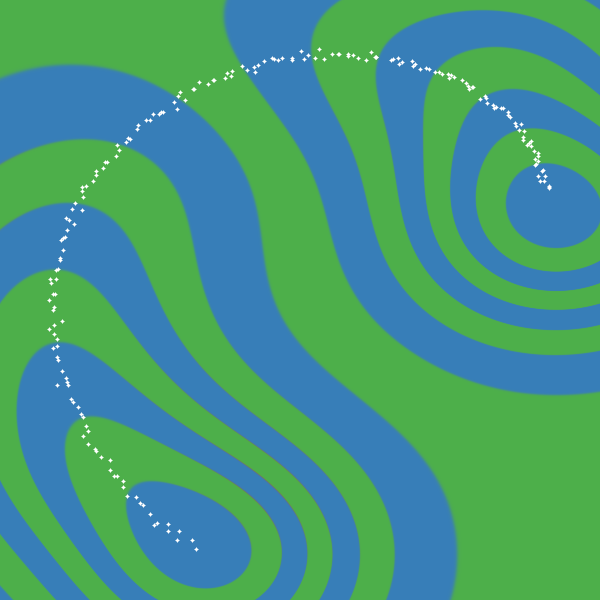
\includegraphics[width=0.45\columnwidth]{\deeplimitsfiguresdir/hidden_good} &
\begin{tikzpicture}[pile/.style={thick, ->, >=stealth'}]
    \node[anchor=south west,inner sep=0] at (0,0) {
    	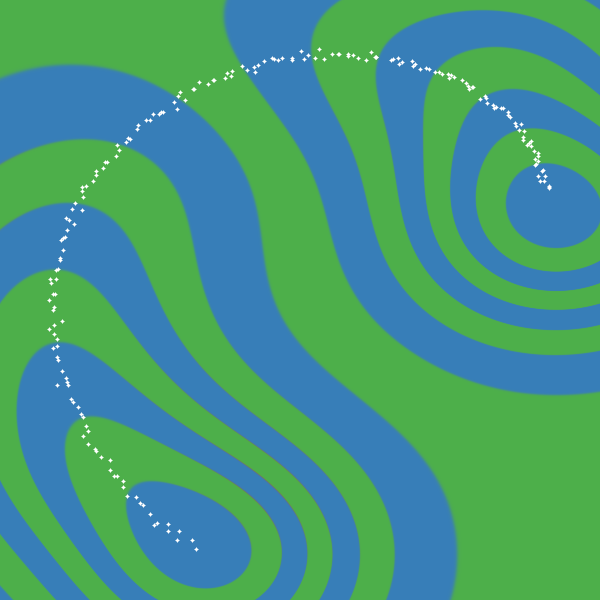
\includegraphics[clip, trim = 0cm 12cm 0cm 0.0cm, width=0.9\columnwidth]{\deeplimitsfiguresdir/hidden_good}
    };
    \coordinate (D) at (1.6,1.5);
    \coordinate (Do) at (2.1,0.9);
    \coordinate (Dt) at (2.8,2.4);
    
    \draw[pile] (D) -- (Dt) node[right, text width=5em] { tangent };
    \draw[pile] (D) -- (Do) node[right, text width=5em] { orthogonal };
\end{tikzpicture}
%A noise-tolerant representation  of \\ a one-dimensional manifold (white)
%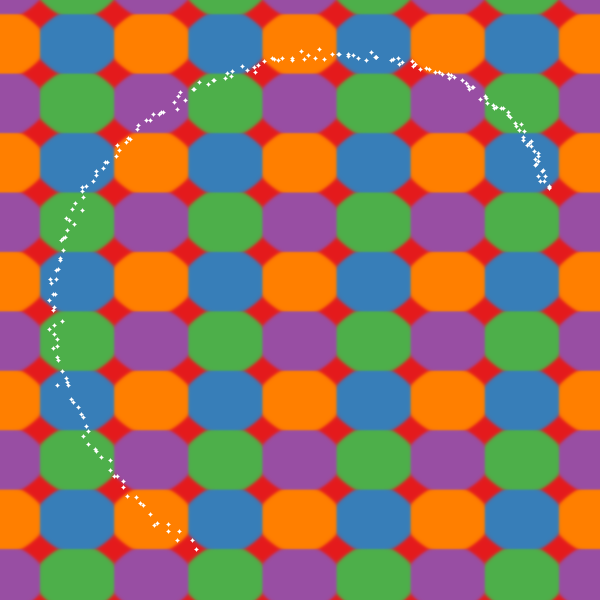
\includegraphics[clip, trim = 0cm 12cm 0cm 0.0cm, width=0.9\columnwidth]{\deeplimitsfiguresdir/hidden_bad} \\
%b) A na\"{i}ve representation (colors) \\ of a one-dimensional manifold (white)
%\end{tabular}
\caption[Desirable properties of representations of manifolds]
{Representing a 1-D manifold.
%A representation is a function mapping the input space to some set of outputs.
Colors show the output of the computed representation as a function of the input space.
The representation (blue \& green) is invariant in directions orthogonal to the data manifold (white), making it robust to noise in those directions, and reducing the number of parameters needed to represent a datapoint.
The representation also changes in directions tangent to the manifold, preserving information for later layers. 
%Representation b) changes in all directions, preserving potentially useless information.}% The representation on the right might be useful if the data were spread out in over plane.
}
\label{fig:hidden}
\end{figure}
%
We follow \cite{rifai2011contractive} in characterizing the representational properties of a function by the singular value spectrum of the Jacobian. In their experiments, the Jacobian was computed at the training points.  Because the priors we are examining are stationary, the distribution of the Jacobian is identical everywhere.
%
\newcommand{\spectrumpic}[1]{
%\hspace{-0.2in}
\includegraphics[trim=4mm 1mm 4mm 2.5mm, clip, width=0.475\columnwidth]{\deeplimitsfiguresdir/spectrum/layer-#1}} 
\begin{figure}[t]
\centering
\begin{tabular}{ccc}
& 2 layers & 6 layers \\
\hspace{-0.3cm} \begin{sideways} {\scriptsize \quad Normalized singular value} \end{sideways} & \hspace{-0.2in} \spectrumpic{2} & \hspace{-0.2in} \spectrumpic{6} \\
 & {\footnotesize Singular value index} & {\footnotesize Singular value}
\end{tabular}
\caption[Singular value spectrum of the Jacobian of a deep GP]
{The normalized singular value spectrum of the Jacobian of a deep GP.  As the net gets deeper, the largest singular value dominates.
This implies that with high probability, there is only one effective degree of freedom in the representation being computed.
%As depth increases, the distribution on singular values also becomes heavy-tailed.
}
\label{fig:deep_spectrum}
\end{figure}
%
\begin{figure}[h!]
\centering
\begin{tabular}{cc}
$p(\vx)$ & $p(\vf^{(1)}(\vx))$ \\
\gpdrawbox{1} &
\gpdrawbox{2} \\
$p(\vf^{(1:4)}(\vx))$ &  $p(\vf^{(1:6)}(\vx))$ \\
\gpdrawbox{4} & 
\gpdrawbox{6}
%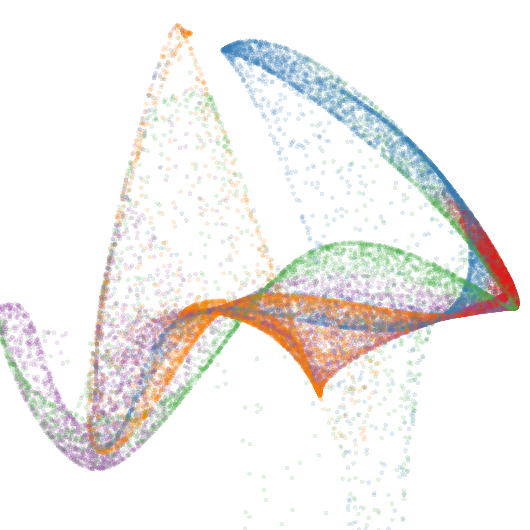
\includegraphics[width=0.3\columnwidth]{\deeplimitsfiguresdir/deep_draws/deep_gp_sample_layer_3} \\
%$p(\vx)$ & $p(f_1(\vx))$ & $p(f_2(f_1(\vx)))$ \\ \\
%\fbox{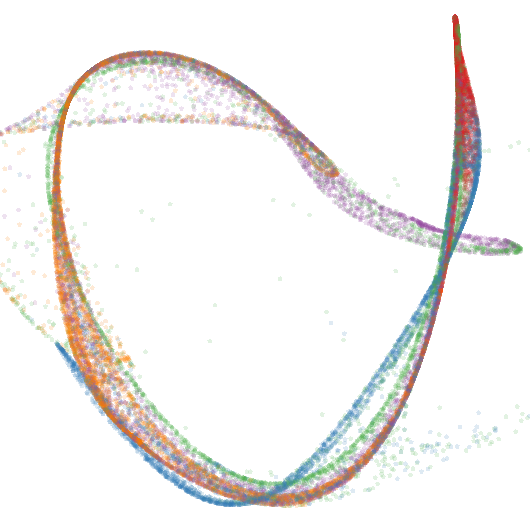
\includegraphics[width=0.24\columnwidth]{\deeplimitsfiguresdir/deep_draws/deep_gp_sample_layer_4}} &
%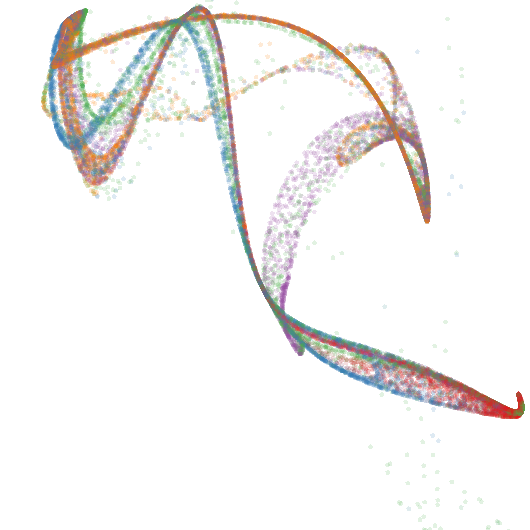
\includegraphics[width=0.3\columnwidth]{\deeplimitsfiguresdir/deep_draws/deep_gp_sample_layer_5} &
%\fbox{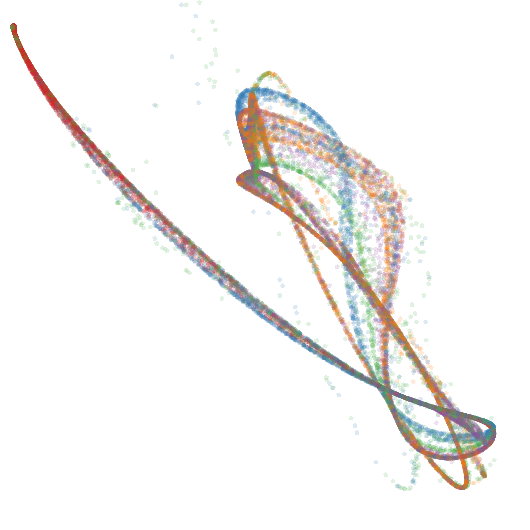
\includegraphics[width=0.24\columnwidth]{\deeplimitsfiguresdir/deep_draws/deep_gp_sample_layer_6}} \\
%$p(f_3(f_2(f_1(\vx))))$ & $p(f_4(f_3(f_2(f_1(\vx)))))$ & $p(f_5(f_4(f_3(f_2(f_1(\vx)))))$
%density of $\vf^{(1:4)}(\vX))$ & density of $\vf^{(1:6)}(\vX))$
\end{tabular}
\caption[Visualization of draws from a deep GP]
{Visualization of draws from a deep GP.
A 2-dimensional Gaussian distribution (top left) is warped by successive functions drawn from a GP prior.
As the number of layers increases, the density concentrates along one-dimensional filaments.}
\label{fig:filamentation}
\end{figure}
%
Figure \ref{fig:deep_spectrum} shows the singular value spectrum for 5-dimensional deep GPs of different depths.  As the net gets deeper, the largest singular value dominates, implying there is usually only one effective degree of freedom in representation being computed.
%


Figure \ref{fig:filamentation} demonstrates a related pathology that arises when composing functions to produce a deep density model.  The density in the observed space eventually becomes locally concentrated onto one-dimensional manifolds, or \emph{filaments}, implying that such models are insuitable to model manifolds whose underlying dimensionality is greater than one.

\newcommand{\mappic}[1]{\hspace{-0.05in}\includegraphics[width=0.465\columnwidth]{\deeplimitsfiguresdir/map/latent_coord_map_layer_#1}} 
\newcommand{\mappiccon}[1]{\hspace{-0.05in} \includegraphics[width=0.465\columnwidth]{\deeplimitsfiguresdir/map_connected/latent_coord_map_layer_#1}}
\begin{figure}[h!]
\centering
\begin{tabular}{cc}
Identity Map: $\vy = \vx$ & 1 Layer: $\vy = f^{(1)}(\vx)$ \\
\mappic{0} & \mappic{1} \\
 2 Layers: $\vy = f^{(1:2)}(\vx)$ & 10 Layers: $\vy = f^{(1:10)}(\vx)$ \\%\\2 Layers: $\vy = f_1(f_2(\vx))$ \\
\mappic{2} & \mappic{10}
%\begin{tikzpicture}[pile/.style={thick, ->, >=stealth'}]
%    \node[anchor=south west,inner sep=0] at (0,0) {
%    	\mappic{40}
%    };
%    \coordinate (D) at (0.3,1.4);
%    \coordinate (Dt) at (1.3,2.4); 
%    \draw[pile, white] (D) -- (Dt) node[right, text width=5em] {};
%\end{tikzpicture}
\end{tabular}
\caption[Feature mapping of a deep GP]
{Feature mapping of a deep GP.
Colors correspond to the location $\vy = \vf(\vx)$ that each point is mapped to after being warped by a deep GP.
%This figure can be seen as the inverse of figure \ref{fig:filamentation}.  
The number of directions in which the color changes rapidly corresponds to the number of large singular values in the Jacobian.
Just as the densities in figure \ref{fig:filamentation} became locally one-dimensional, there is usually only one direction that one can move $\vx$ in locally to change $\vy$.
This means that $\vf$ is unlikely to be a suitable representation for decision tasks that depend on more than one aspect of $\vx$.}
\label{fig:deep_map}
\end{figure}
%
To visualize this pathology in another way, figure \ref{fig:deep_map} illustrates a colour-coding of the representation computed by a deep \gp{}, evaluated at each point in the input space.  After 10 layers, we can see that locally, there is usually only one direction that one can move in $\vx$-space in order to change the value of the computed representation.  This means that such representations are likely to be unsuitable for decision tasks that depend on more than one property of the input.

To what extent are these pathologies present in nets being used today?  In simulations, we found that for deep functions with a fixed latent dimension $D$, the singular value spectrum remained relatively flat for hundreds of layers as long as $D > 100$.  Thus, these pathologies are unlikely to severely affect relatively shallow, wide networks.

%This pathology stems from the independence of the layer-wise transformations.  Because
%As such, in the limit of the network depth approaching infinity, with probability 1 there exists at most a single eigenvalue with magnitude greater than zero, as was suggested by our empirical observations.





\section{Fixing the pathology}
\label{sec:fix}

\begin{figure}[h!]
\def\layersep{1.33cm}
\def\nodeseptwo{1.8cm}
\def\nodesize{.35cm}

\begin{tabular}{c}
\bardist
\begin{tikzpicture}[draw=black!80]
    \tikzstyle{neuron}=[circle,minimum size=17pt, draw = black!80, fill = white, thick]
    \tikzstyle{input neuron}=[neuron, fill=green!50];
    \tikzstyle{output neuron}=[neuron, fill=red!50];
    \tikzstyle{hidden neuron}=[neuron, fill=blue!50];
    \tikzstyle{pile} =[thick, ->, >=stealth', shorten <=7pt, shorten >=8pt];

    % Define the input layer node
    \coordinate (I) at (0, 0);


    % Define the hidden layer nodes
    \foreach \name / \y in {1,...,\numhidden}
    {
        \coordinate (H-\name) at (\nodeseptwo*\y, 0);
    }

    % Connect every node            
    \foreach \name in {1,...,\numhidden}
    {
	 \path[pile] (I) edge (H-\name) {};
         %\path[pile] (I) edge [bend left] (H-\name) {};
    }

    \draw (I) node[neuron] {};
    \draw (I) node[below = 0.5cm]  {$\vx$};

    % Draw the hidden layer nodes
    \foreach \name / \y in {1,...,\numhidden}
    {
	\draw (H-\name) node[neuron]  {};
        \draw (H-\name) node[below = 0.34cm] {$\vf^{(\y)}(\vx)$};
    }
\end{tikzpicture} \\
a) The standard \MLP{} connectivity architecture. \\
\bardist
\begin{tikzpicture}[draw=black!80]
    \tikzstyle{neuron}=[circle,minimum size=17pt, draw = black!80, fill = white, thick]
    \tikzstyle{input neuron}=[neuron, fill=green!50];
    \tikzstyle{output neuron}=[neuron, fill=red!50];
    \tikzstyle{hidden neuron}=[neuron, fill=blue!50];
    \tikzstyle{pile} =[thick, ->, >=stealth', shorten <=7pt, shorten >=8pt];

    % Define the input layer node
    \coordinate (I) at (0, 0);


    % Define the hidden layer nodes
    \foreach \name / \y in {1,...,\numhidden}
    {
        \coordinate (H-\name) at (\nodeseptwo*\y, 0);
    }

    % Connect every node
    \path[pile] (I) edge (H-1) {};          
    \foreach \name in {2,...,\numhidden}
    {
	 \path[pile] (I) edge (H-\name) {};
         \path[pile] (I) edge [bend left] (H-\name) {};
    }

    \draw (I) node[neuron] {};
    \draw (I) node[below = 0.5cm]  {$\vx$};

    % Draw the hidden layer nodes
    \foreach \name / \y in {1,...,\numhidden}
    {
	\draw (H-\name) node[neuron]  {};
        \draw (H-\name) node[below = 0.34cm] {$\vf^{(\y)}(\vx)$};
    }
\end{tikzpicture} \\
b) Input-connected architecture.
\end{tabular}
\caption[Two different architectures for deep neural networks]
{Two different architectures for deep neural networks.
The standard architecture connects each layer's outputs to the next layer's inputs.
The input-connected architecture also connects the original input $\vx$ to each layer.}
\label{fig:input-connected}
\end{figure}


Following a suggestion from \cite{neal1995bayesian}, we can fix the pathologies exhibited in figures \ref{fig:filamentation} and \ref{fig:deep_map} by simply making each layer depend not only on the output of the previous layer, but also on the original input $\vx$.  
We refer to these models as \emph{input-connected} networks.
Figure \ref{fig:input-connected} shows a graphical representation of the two connectivity architectures.
Similar connections between non-adjacent layers can also be found the primate visual cortex \citep{maunsell1983connections}.
Formally, this functional dependence can be written as
\begin{align}
\vf^{(1:L)}(\vx) = \vf^{(L)} \left( \vf^{(1:L-1)}(\vx), \vx \right), \quad \forall L
\end{align}
%
Draws from the resulting prior are shown in figures \ref{fig:deep_draw_1d_connected}, \ref{fig:no_filamentation} and \ref{fig:deep_map_connected}.
%
\begin{figure}[t]
\centering
\begin{tabular}{cccc}
\hspace{-0.1in} One layer & \hspace{-0.2in} 2 Layers & \hspace{-0.2in}  5 Layers & \hspace{-0.25in} 10 Layers \\
\hspace{0.03in}
\onedsamplepiccon{1} &
\onedsamplepiccon{2} &
\onedsamplepiccon{5} &
\onedsamplepiccon{10}
%& 6 layers \\ & largest , for unconnected layers & largest, for connected layers
\end{tabular}
\caption[Draws from a 1D deep GP prior with each layer connected to the input]
{Draws from a 1D deep GP prior with each layer connected to the input.
Even after many layers, the functions remain smooth in some regions, while varying rapidly in other regions.
Compare to standard-connectivity deep GP draws shown in figure \ref{fig:deep_draw_1d}.}
\label{fig:deep_draw_1d_connected}
\end{figure}
%
%Figure \ref{fig:deep_draw_1d_connected} shows draws from a 1D deep \gp{} prior with a connected architecture.
%
%\begin{figure}
%\centering
%\begin{tabular}{ccc}
%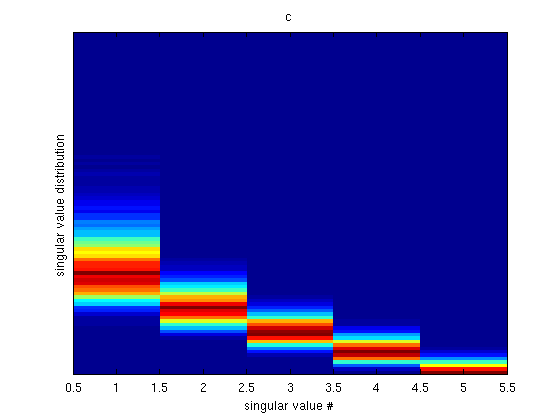
\includegraphics[width=0.3\columnwidth]{\deeplimitsfiguresdir/spectrum/svd_specturm_depth_50_connected} &
%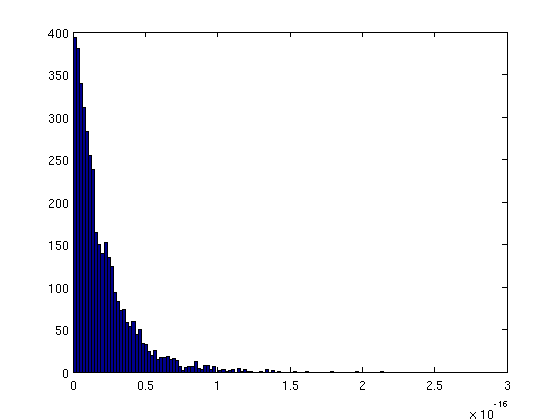
\includegraphics[width=0.3\columnwidth]{\deeplimitsfiguresdir/spectrum/svd_ratio_depth_50} &
%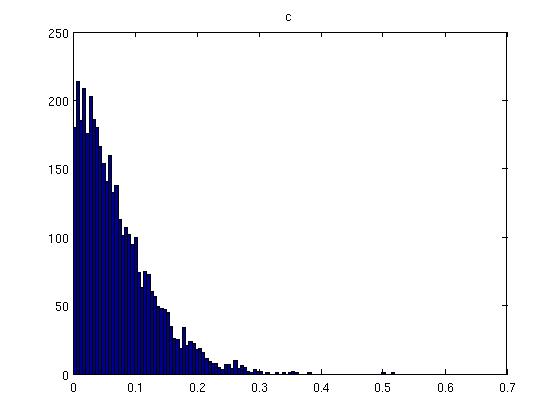
\includegraphics[width=0.3\columnwidth]{\deeplimitsfiguresdir/spectrum/svd_ratio_depth_50_connected} \\
%50 connected layers & smallest singular value divided by & 6 layers \\
% & largest , for unconnected layers & largest, for connected layers
%\end{tabular}
%\caption{Reparing the singular value distribution.  When each layer is connected to the original inputs, and the variance of derivatives is smaller than a threshold, then the ratio of the largest singular value to the smallest remains small.}
%\label{fig:deep_spectrum_fixed}
%\end{figure}
%
%
\newcommand{\gpdrawboxcon}[1]{
\setlength\fboxsep{0pt}
\hspace{-0.2in} 
\fbox{
\includegraphics[width=0.464\columnwidth]{\deeplimitsfiguresdir/deep_draws_connected/deep_sample_connected_layer#1}
}}
%
\begin{figure}[h!]
\centering
\begin{tabular}{cc}
%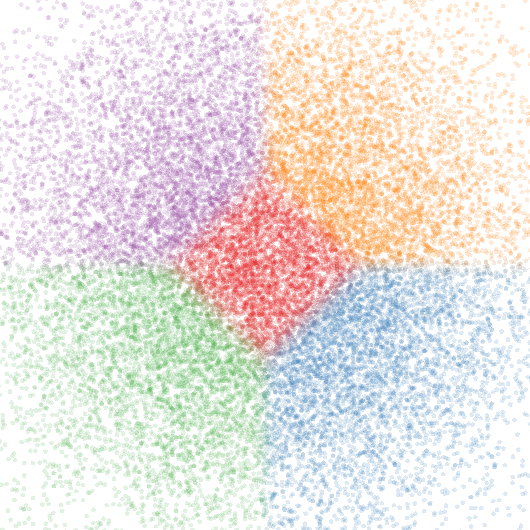
\includegraphics[width=0.3\columnwidth]{\deeplimitsfiguresdir/deep_draws/deep_gp_sample_layer_1} &
%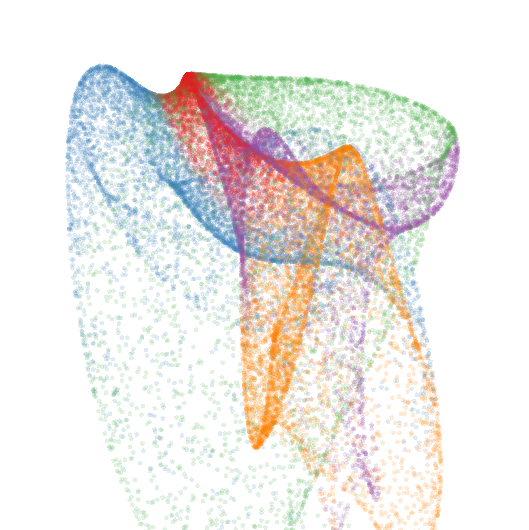
\includegraphics[width=0.3\columnwidth]{\deeplimitsfiguresdir/deep_draws_connected/deep_sample_connected_layer2} &
%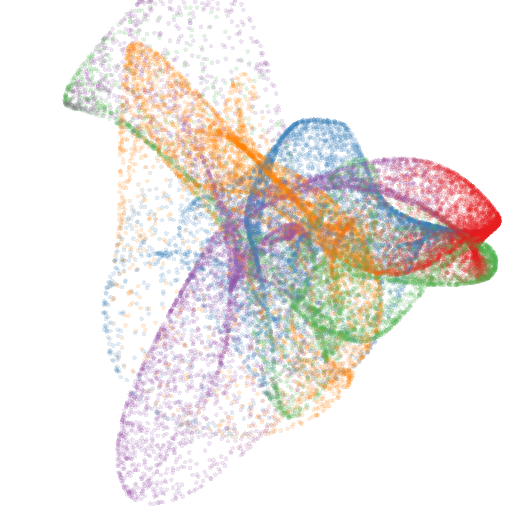
\includegraphics[width=0.3\columnwidth]{\deeplimitsfiguresdir/deep_draws_connected/deep_sample_connected_layer3} \\
%$p(\vx)$ & $p(f_1(\vx))$ & $p(f_2(f_1(\vx), \vx))$ \\ \\
%\gpdrawboxcon{2} &
3 Layers & 6 Layers \\
\gpdrawboxcon{3} &
\gpdrawboxcon{6}
\end{tabular}
\caption[Densities defined by a draw from a deep GP]
{Left: Densities defined by a draw from a deep GP, with each layer connected to the input $\vx$.
As depth increases, the density becomes more complex without concentrating along filaments.}
\label{fig:no_filamentation}
\end{figure}
%
%\begin{tabular}{c}
%
%\gpdrawboxcon{6} \\
%$p(f_3(f_2(f_1(\vx),\vx),\vx))$ & $p(f_4(f_3(f_2(f_1(\vx), \vx),\vx),\vx))$ & $p(f_5(f_4(f_3(f_2(f_1(\vx),\vx),\vx),\vx),\vx))$
\begin{figure}[h!]
\centering
\newcommand{\spectrumpiccon}[1]{
\includegraphics[trim=4mm 1mm 4mm 2.5mm, clip, width=0.475\columnwidth]{\deeplimitsfiguresdir/spectrum/con-layer-#1}} 
\begin{tabular}{ccc}
 & 25 layers &  50 layers \\
\hspace{-0.5cm} \begin{sideways} {\scriptsize \quad Normalized singular value} \end{sideways} & \hspace{-0.2in} \spectrumpiccon{25} & \hspace{-0.16in} \spectrumpiccon{50} \\
 & {\scriptsize Singular value number} & {\scriptsize Singular value number}
\end{tabular}
\caption[Distribution of singular values of an input-connected deep GP]
{The distribution of singular values drawn from 5-dimensional input-connected deep GP priors 25 and 50 layers deep.
The singular values remain roughly the same scale as one another.}
\label{fig:good_spectrum}
\end{figure}
%
%
\begin{figure}[h!]
\centering
\begin{tabular}{cc}
Identity map: $\vy = \vx$ & 2 Connected layers \\
\hspace{-0.07in} \mappic{0} & \mappiccon{2} \\
 10 Connected layers & 20 Connected layers \\
\hspace{-0.07in} \mappiccon{10} & \mappiccon{20}
\end{tabular}
\caption[Feature mapping of an input-connected deep GP]
{Feature mapping of a deep GP with each layer connected to the input $\vx$.
Just as the densities in figure \ref{fig:no_filamentation} remained locally two-dimensional even after many transformations, in this mapping there are often two directions that one can move locally in $\vx$ to in order to change the values of $\vf(\vx)$.
This means that the prior puts mass on representations which sometimes depend on all aspects of the input.
Compare to figure \ref{fig:deep_map}.
}
\label{fig:deep_map_connected}
\end{figure}
%
%
%
%\paragraph{Jacobian of input-connected deep networks}
The Jacobian of the composed, input-connected deep function is defined by the recurrence
%
\newcommand{\sbi}[2]{\left[ \! \begin{array}{c} #1 \\ #2 \end{array} \! \right]} 
%\newcommand{\sbi}[2]{\left[ #1 \quad \!\! #2 \right]} 
\begin{align}
{J^{1:L}(\vx) = J^L \sbi{ J^{1:L-1}}{I_D}}.
\end{align}
%
%So the entire Jacobian has the form:
%
%\begin{align}
%J^{1:L}(x) = J^L \sbi{ J^{L-1} \sbi{ \dots J^{4} \sbi{ J^{3} \sbi{ J^2 J^1 }{ I_D }}{ I_D } \dots }{ I_D \\ %\vdots }}{ I_D}
%\end{align}
%
Figure \ref{fig:good_spectrum} shows that with this architecture, even 50-layer deep \gp{}s have well-behaved singular value spectra.

%Connecting the input to each layer is a simple method to correct the pathology exhibited, but it may not

%\subsection{Other refinements}

%The input-connected architecture fixes the pathology described above





\section{Related work}

Deep \gp{}s were first proposed by \cite{lawrence2007hierarchical}. Variational inference in deep \gp{}s was developed by \cite{damianou2012deep}, who also analyzed the effect of automatic relevance determination in that model.

%Other Bayesian deep neural network models have been proposed by, for example, . % and Sum-product networks \cite{poon2011sum}  
\citet{adams2010learning} proposed a prior on deep Bayesian networks.  Their architecture has no connections except between adjacent layers, and may also be expected to have similar pathologies as deep \gp{}s as the number of layers increases.
%
Deep Density Networks \citep{rippel2013high} were constructed with invertibility in mind, with penalty terms encouraging the preservation of information about lower layers. Such priors are a promising approach to alleviating the pathology discussed in this paper.

\paragraph{Recurrent networks}
\cite{bengio1994learning} and \cite{pascanu2012understanding} analyze a related problem with gradient-based learning in recurrent nets, the ``exploding-gradients'' problem.
\cite{hermans2012recurrent} analyze deep kernels corresponding to recurrent neural networks.

\paragraph{Analysis of deep learning}
\cite{montavon2010layer} perform a layer-wise analysis of deep networks, and note that the performance of MLPs degrades as the number of layers with random weights increases.
The importance of network architectures relative to learning has been examined by \cite{saxe2011random}.
\cite{saxedynamics} looked at the dynamics of learning in deep linear models, as a tractable approximation to deep neural networks.  




%\section{Discussion}


%\paragraph{Recursive learning method}
%Just as layer-wise unsupervised pre-training encourages the projection of the data into a representation with independent features in the higher layers, so does the procedure outlined here.  This is because the isotropic kernel does not penalize independence between different dimensions, only the number of dimensions.





\section{Conclusions}

%In this work, we established a number of propositions which help us gain insight into the properties of very deep models, and allow making informed choices regarding their architecture.

In this work, we attempted to gain insight into the properties of deep neural networks by characterizing the sorts of functions likeley to be obtained under different choices of priors on compositions of functions.
%established a number of propositions which help us gain insight into the properties of very deep models, and allow making informed choices regarding their architecture.

%First, we identified equivalences between multi-layer perceptions and deep \gp{}s --- namely, that a deep \gp{} can be written as an \MLP{}s with a finite number of nonparametric hidden units, or as an \MLP{} with infinitely-many parametric hidden units.
First, we identified deep Gaussian processes as an easy-to-analyze model corresponding to multi-layer preceptrons with nonparametric activation functions.
%  We also showed several other connections between deep \MLP{}s and different Gaussian process models. %equivalences between multi-layer perceptions and deep \gp{}s --- namely, that a deep \gp{} can be written as an \MLP{}s with a finite number of nonparametric hidden units, or as an \MLP{} with infinitely-many parametric hidden units.
%
%Second, we characterized the derivatives and Jacobians of deep \gp{}s through products of independent Gaussian matrices. % can be characterized using random matrix theory, which we applied to establish results regarding the distribution over the Jacobian of the composition transformation. 
We then showed that representations based on repeated composition of independent functions exhibit a pathology where the representations becomes invariant to all directions of variation but one. % This leads to extremely restricted expressiveness of such deep models in the limit of increasing number of layers. 
Finally, we showed that this problem could be alleviated by connecting the input to each layer.
%proposed a way to alleviate this problem: connecting the input to each layer of a deep representation allows us to construct priors on deep functions that do not exhibit the information-capacity pathology.

We also examined properties of deep kernels, corresponding to arbitrarily many compositions of fixed features.
Finally, we derived models obtained by performing dropout on Gaussian processes, finding a tractable approximation to exact dropout in \gp{}s.




\outbpdocument{
%This will be ignored, it's just so that Gummi can find the bibliography.
\bibliographystyle{plainnat}
\bibliography{references.bib}
qwerty
}

